\documentclass[tikz]{standalone}

\colorlet{FilledSurface}{blue!20}
\colorlet{FilledSurfaceGroupOne}{blue!20}
\colorlet{FilledSurfaceGroupTwo}{red!20}
\colorlet{FilledSurfaceGroupThree}{green!20}
\colorlet{FilledSurfaceGroupFour}{magenta!20}
\colorlet{FormulaBackground}{green!10}
\colorlet{FormulaFrame}{green}


\usetikzlibrary{calc, decorations.markings, intersections}

\tikzset{
    mark rect/.style={
        decoration={markings, mark=at position 0.5 with {
            \draw[fill=white] (-6pt,-2pt) rectangle (6pt,2pt);
        }}, postaction={decorate}
    },
    mark two circles/.style={
        decoration={markings, mark=at position 0.5 with {
                \draw[fill=white] (-2pt,0) circle (2pt);
                \draw[fill=white] (2pt,0) circle (2pt);
        }}, postaction={decorate}
    }
}

\begin{document}
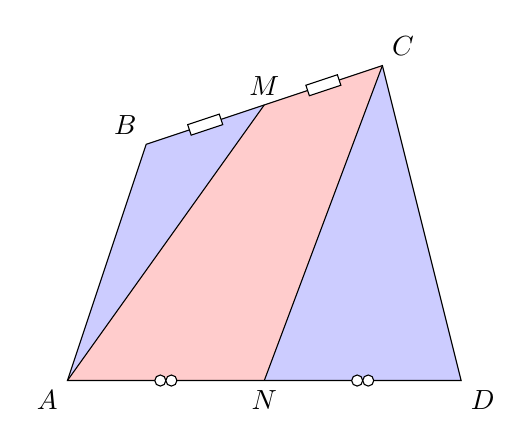
\begin{tikzpicture}

\coordinate (A) at (0, 0);
\coordinate (B) at (1, 3);
\coordinate (C) at (4, 4);
\coordinate (D) at (5, 0);

% Hallar puntos medios de cada lado del cuadrilátero.
\coordinate (M) at ($(B)!0.5!(C)$);
\coordinate (N) at ($(D)!0.5!(A)$);

% Dibujar medianas y nombrar los puntos medios de cada lado.
\draw
(M) node [above] {$M$}
(N) node [below] {$N$}
-- cycle;

% Colorear superficie.
\draw[draw=none, fill=FilledSurfaceGroupOne] (A) -- (B) -- (C) -- (D) -- cycle;
\draw[draw=none, fill=FilledSurfaceGroupTwo] (A) -- (M) -- (C) -- (N) -- cycle;

% Dibujamos los segmentos, luego de colorear las superficies para
% evitar que las superficies cubran a los segmentos.

% Dibujar cuadrilátero
\draw
    (A) node[below left]{$A$}
    -- (B) node[above left]{$B$}
    -- (C) node[above right]{$C$}
    -- (D) node[below right]{$D$}
    -- cycle;

\draw (A) -- (M);
\draw (C) -- (N);

% Añadir marcadores a los segmentos determinados por las medianas.
\path[mark rect] (B) -- (M);
\path[mark rect] (C) -- (M);
\path[mark two circles] (A) -- (N);
\path[mark two circles] (D) -- (N);


\end{tikzpicture}
\end{document}
